%!TEX root = ../main.tex

\section{Вычислительный эксперимент}

\begin{frame}{Параметры модели}
\vspace{-1cm}
\begin{itemize}
	\item Параметры, отражающие реальный физический эксперимент:
\end{itemize}
\centering
\begin{tabular}{|l|c|l|}
	\hline
	Название & Переменная & Значение \\
	\hline
	электрическое напряжение		& $|\nabla \Phi|$	& $5.625 \cdot 10^6 \; \unitV / \unitm$							\\
	энергия роста канала			& $\Gamma$			& $8.118 \cdot 10^{-10} \; \unitJ / \unitm$						\\
	диэлектрическая проницаемость	& $\epsilon_0$		& $2.301 \cdot 10^{-11} \; \unitC^2 / (\unitJ \cdot \unitm)$	\\
	подвижность						& $m$				& $12 \; \unitm^3 / (\unitJ \cdot \units)$						\\
	\hline
	толщина границы					& $l$ 				& $1.5 \cdot 10^{-6} \; \unitm$									\\
	регуляризующий параметр 		& $\delta$			& $10^{-3}$														\\
	размер образца					& $L$				& $3.2 \cdot 10^{-5} \; \unitm$									\\
	продолжительность				& $T$				& $2 \cdot 10^{-3} \; \units$									\\
	шаг по пространству				& $h$				& $5 \cdot 10^{-7} \; \unitm$									\\
	минимальный шаг по времени		& $\tau_{min}$		& $10^{-10} \; \units$											\\
	максимальный шаг по времени		& $\tau_{max}$		& $\leqslant 6.42 \cdot 10^{-6} \; \units$						\\
	\hline
\end{tabular}
\end{frame}


\begin{frame}{Поведение системы}
\vspace{-0.4cm}
\begin{figure}
	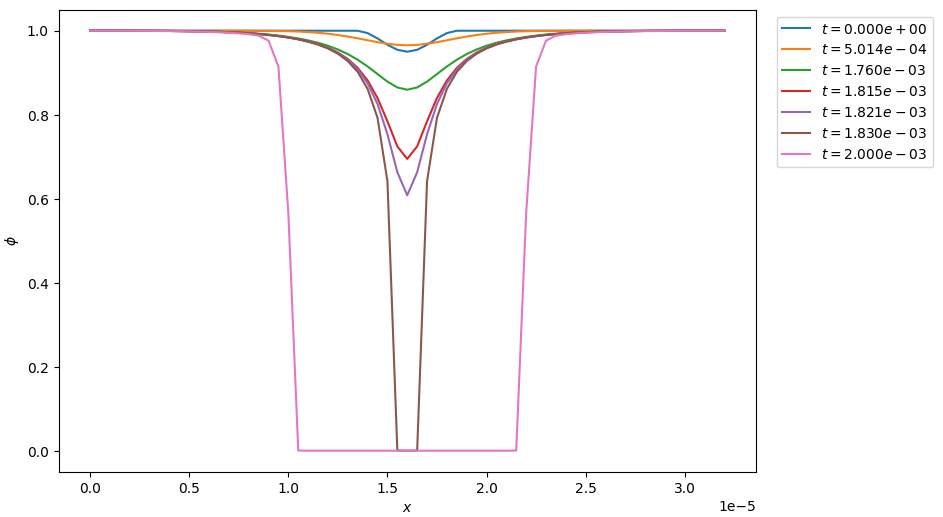
\includegraphics[width=0.87\textwidth]{figures/system_behaviour.png}
\end{figure}
\end{frame}


\begin{frame}{Результаты расчетов}
\centering
\begin{tabular}{|l|c|c|c|}
	\hline
	Тип адаптации & Ускорение (раз) & Отклонение по $\phi$ & Запаздывание \\
	\hline \hline
	по фазовому полю	& 800	& $3.64 \cdot 10^{-4}$	& $0.3\%$		\\
	по энергии			& 107	& $5.38 \cdot 10^{-4}$	& $0.36\%$		\\
	по устойчивости		& 1474	& $1.54 \cdot 10^{-2}$	& $0.71\%$		\\
	\hline \hline
	по фазовому полю	& 101	& $1.23 \cdot 10^{-5}$	& $0.004\%$		\\
	по энергии			& 101	& $3.27 \cdot 10^{-4}$	& $0.19\%$		\\
	по устойчивости		& 100	& $2.23 \cdot 10^{-5}$	& $0.0046\%$	\\
	\hline
\end{tabular}
\end{frame}